\documentclass[10pt,a4paper,ngerman]{scrartcl}
\usepackage[utf8]{inputenc}
\usepackage[ngerman]{babel}

%
\usepackage{fancyref}
\usepackage{geometry}
\usepackage{fancyhdr} 
\usepackage{url}
\usepackage{makeidx}
\usepackage{listings}
\usepackage[utf8]{inputenc}
\usepackage[T1]{fontenc}
\usepackage{lmodern}
\usepackage{amsmath}
\usepackage{setspace}
\usepackage{subfig}
\usepackage{fancyvrb}
\usepackage{bbding}
\usepackage[table]{xcolor}
\usepackage{varwidth}
\usepackage{rotating}
\usepackage{tabularx}
\usepackage{float}
\usepackage{cite}
\usepackage{color}
\usepackage{tocstyle}
\newtocstyle[KOMAlike][leaders]{alldotted}{}
\usetocstyle{alldotted}
\usepackage{todonotes}

\geometry{a4paper, top=25mm, left=35mm, right=20mm, bottom=30mm,
headsep=10mm, footskip=12mm}
%
% PDF settings
\usepackage[pdfstartview=FitH,pdftitle={Ausarbeitung Moderne Web-Technologien},pdfauthor={Jan Bernoth, Sascha Kretzschmann}, colorlinks=false, linktocpage, pdfborder={0 0 0}]{hyperref}

%
% Header and Footer Style
\pagestyle{fancy}
\fancyhead{}
\fancyhead[R]{\slshape Jan Bernoth - Sascha Kretzschmann}
\fancyhead[L]{\slshape\nouppercase{\rightmark}}
\fancyfoot{}
\fancyfoot[C]{\thepage}
\renewcommand{\headrulewidth}{0pt}
\renewcommand{\sectionmark}[1]{\markright{\thesection\ #1}} 
%
% No identation
\setlength\headheight{15pt}
\setlength\parindent{0pt} 
%
% Custom commands
\newcommand\zb{z.\,B.\ }
\renewcommand\dh{d.\,h.\ }
\newcommand\parbig{\par\bigskip}
\newcommand\parmed{\par\medskip}
\newcommand{\mailto}[1]{\href{mailto:#1}{#1}}
%
% Misc
\DeclareGraphicsExtensions{.pdf}
\graphicspath{{pictures/}}
%
% Titel and author 
\title{
\includegraphics[width=0.6\textwidth]{pictures/logo}\\
{\normalsize Seminar Moderne Web-Technologien\\
Arbeitsgruppe Netzbasierte Informationssysteme}\\[9ex]
Einführung in SVG\\}
\author{Jan Bernoth\\{janbernoth@gmail.com}\and Sascha Kretzschmann\\{s.kretzschmann@fu-berlin.de}\\\\}
\date{\today}

\begin{document}
\pagenumbering{arabic}

\maketitle
\thispagestyle{empty}
\newpage

\Large{\textbf{\emph{Abstract}}}
\begin{abstract}
Die vorliegende Ausarbeitung zum Thema Scalable Vector Graphics (SVG) dient als Einführung in den vom World Wide Web Consortium (W3C) veröffentlichten Standard für skalierbare Vektorgrafiken und ist im Zusammenhang mit dem Seminar Moderne Webtechnologien an der Freien Universität Berlin im Wintersemester 2014/2015 entstanden.\\
Im ersten Teil werden grundlegende Ideen, Strukturen und Konzepte zur Arbeit mit SVG beschrieben und anhand zahlreicher Beispiele visualisiert.\\
Der zweite Teil beinhaltet erweiterte Konzepte und stellt mögliche Anwendungen von SVG vor.\\
Zum Schluss wird ein Ausblick auf SVG 2.0 dargestellt, welcher als Nachfolger der aktuellen Version angesehen wird und die Beschreibung des kleinen Projektes, welches im Verlauf der Arbeit mit SVG entstanden ist.
\end{abstract}

\newpage
\tableofcontents
%\listoffigures
%\listoftables
\newpage

\section{Idee und Renderingmodell}
\subsection{Über SVG}
SVG wurde im September 2001 vom W3C veröffentlich und stellt eine empfohlene Spezifikation für zweidimensionale Vektorgrafiken bereit. Die aktuelle Version 1.1 wurde als W3C Recommendation am 14.Januar 2003 veröffentlicht und dient als Grundlage dieser Ausarbeitung \cite{svg:2003}.\\
Sie basiert auf der Auszeichnungssprache XML \cite{xml:2008}.\\
In diesem Kapitel soll kurz die Idee hinter SVG, sowie dessen Renderingmodell skizziert werden.

\subsection{Grundlegende Konzepte}
Hinter der Abkürzung SVG, also Scalable Vector Graphics (dt. skalierbare Vektorgrafiken), stehen mehrere Ideen und grundlegende Konzepte, die mit dem Standard umgesetzt werden sollen.\\

\textit{Skalierbar}\\
Der Begriff skalierbar bezieht sich auf zwei Dimensionen. Zum einen ist es eine Eigenschaft der Grafiken. Unabhängig der möglichen Auflösung eines Endgerätes, soll diese Art der Grafiken immer gleich scharf abgebildet werden. Auch bei Vergrößerungs- und Verkleinerungseffekten gibt es bei Vektorgrafiken keinen Qualitätsverlust.
Der zweite Aspekt betrifft die Skalierbarkeit im Web allgemein, da es mit anderen Standards problemlos integriert werden kann.\\

\emph{Vector}\\
Grafiken in SVG bestehen ausschließlich aus geometrischen Objekten, wie Linien und Kurven. Dadurch wird eine größere Flexibilität im Vergleich zu Rastergrafiken erzeugt, in denen alle Informationen in den einzelnen Pixeln gespeichert sind.\\

\emph{Graphics}\\
SVG sollte die Lücke zwischen XML, mit rein textuellen Informationen bzw. Rohdaten, und HTML schließen, dessen grafische Raffinesse sich damals beinahe ausschließlich auf das \texttt{<image>}-Tag beschränkte.

 
\subsection{Renderingmodell}
Das Renderingmodell kann sehr detailliert betrachtet werden. An dieser Stelle soll es jedoch ausreichen, grundlegende Prinzipien kurz zu erläutern.
Alle grafischen Objekte in SVG werden beim Rendern nacheinander folgend auf das Ausgabegerät "gemalt". Dabei belegt jede Operation einen bestimmten, meist vom Ersteller festgelegten, Bereich. Ist an dieser Stelle schon ein anderes Objekt, wird es (teilweise) überdeckt.
Objekte, welche am Anfang des Dokuments definiert wurden, werden auch zuerst gerendert. Enthält ein Objekt untergeordnete Objekte, werden diese auf den Bereich des Elternobjektes angewendet.

\newpage

\section{Aufbau und Syntax}
\subsection{Einleitung}
In diesem Abschnitt werden die wichtigsten Strukturen zum Aufbau eines SVG Dokumentes vorgestellt.
\subsection{Grundlegende Strukturelemente}
\emph{<svg>}\\
 Das \texttt{<svg>}-Tag ist das Grundlegenste. Innerhalb dessen werden alle (grafischen) Eigenschaften eines Dokuments definiert und das beliebig komplex, wobei \texttt{<svg> </svg>} bereits gültig ist. Zu bemerken ist noch, dass durch Attribute einige Eigenschaften der Ergebnisdatei bestimmt werden könne. Zum Beispiel ist es möglich über die Attribute \texttt{width} und \texttt{height} die Breite respektive Höhe des Zeichenbereichs festzulegen.\\
 
\emph{<g>}\\
 Das Gruppenelement \texttt{<g>} kann zum Zusammenfassen von Objekte verwendet werden. Das hat einmal den Vorteil, die Lesbarkeit von SVG Code zu verbessern und zusammenhängende Strukturen zu verdeutlichen. Weiterhin können gruppierte Objekte gleichzeitig verändert werden, indem nicht jedes einzelne Element angesprochen wird, sondern lediglich die übergeordnete Gruppe. Dabei wird jede Gruppe durch ein \texttt{id}-Attribut identifiziert werden.\\
 
\emph{<symbol>}\\
 Das \texttt{<symbol>} Element ist eine weitere Möglichkeit Objekte zu gruppieren. Es hat die gleichen Eigenschaften, wie das \texttt{<g>} Element. Der wichtigste Unterschied ist, dass Objekte, die mit \texttt{<symbol>} gruppiert sind, erst gerendert werden, wenn sie referenziert werden. Referenzierungen können mit Hilfe des \texttt{<use>} Elements bewerkstelligt werden.
 
 \subsection{Vordefinierte Formen}\label{basic_shapes}
 SVG hat einige grundlegende Formen, die benutzt werden können, um einfache oder zusammengestzte Objekte aufzubauen.\\
 
\emph{Viereck}\\
Mit dem Element \texttt{<rect>} können einfache Vierecke definiert werden. Diese werden über die Attribute Breite (\texttt{width}) und Höhe (\texttt{height}) definiert. Ein einfaches Beispiel befindes sich im Anhang Abbildung\ref{fig:rect}\\

\emph{Kreis}\\
Kreise werden mit \texttt{<circle>} beschrieben. Dabei wird die Größe über das Attribut \texttt{r} (Radius) angegeben (s. Abbildung \ref{fig:circle}).\\

\emph{Ellipse}\\
Das Element \texttt{<elipse>} definiert eine Ellipse, die mit den jeweiligien Radien für die x- und y-Achse definiert werden. Die entsprechenden Attribute sind \texttt{rx} und \texttt{ry} (s. Abbildung \ref{fig:ellipse}).\\

\emph{Polygon}\\
Polygone sind sehr flexible Objekte. Sie werden mit dem Element \texttt{<polygon>} definiert, welches das Attribut \texttt{points} hält. Dieses bekommt eine Anzahl Punkte. So ist es mögliche, beliebige Polygone zu zeichnen. Der letzte Punkt wird automatisch mit dem Startpunkt verbunden, so dass es Polygon entsteht (s. Abbildung \ref{fig:poly}).\\

\emph{Linie}\\
Um eine einfache Linie zu zeichnen, wird das Element \texttt{<line>} benutzt. Es werden nur je zwei Start- und Endpositionen für die y- und x-Achse definiert (s. Abbildung \ref{fig:line}).\\

\emph{Polyline}\\
Eine Polyline wird mit \texttt{<polyline>} beschrieben und ist mit dem Polygon vergleichbar. Auch eine Polyline wird über Punkte definiert mit dem einzigen Unterschied, dass der letzte Punkt nicht mit dem Startpunkt verbunden wird, so dass es sich im Prinzip um ein nicht geschlossenes Polygon handelt (s. Abbildung \ref{fig:polyl}).\\

\emph{Text}\\
Auch Texte können leicht mit SVG dargestellt werden. Dabei wird der darzustellende Text einfach innerhalb des \texttt{<text> </text>} Elements geschrieben. Ein einfaches Beispiel befindet sich im Anhang \ref{fig:text}.

\newpage

\section{Integrierte Grundkonzepte}
\section{Vergleich zwischen SVG Tiny und SVG Mobile}
SVG Tiny und SVG Mobile sind zwei Profile der SVG Full Recommendation. Das heißt, diese beiden Bibliotheken haben Schnittmengen vom SVG, sind jedoch deutlich kleiner als die vollständige Bibliothek. Der Bedarf dazu kam von der Industrie. Diese nutzte das SVG schon innerhalb ihrer Software und brauchten noch eine Lösung für mobile Endgeräte. Anfang der 200er waren die mobilen Endgeräte nicht leistungsfähig genug, um den vollen Umfang des SVG's darstellen zu können. Hinzu kommt, dass die Bibliothek für damalige Verhältnisse einen großen Speicherplatz bedarf. Um diesen Bedarf gerecht zu werden, wurden diese zwei Profile entwickelt.\\

Interessanterweise wird das SVG momentan in der Version 1.1 empfohlen, während das SVG Tiny in der Version 1.2 vorhanden ist. Der Grund dafür liegt im Entwicklungsprozess der SVG Recommendations. Diese wurde weiter entwickelt, sodass einige wenige Fehler verbessert wurden. Aber der neue Funktionsumfang war nicht groß genug, dass sich dafür eine neue Iteration gelohnt hätte. Als Folge entstand lediglich eine neue Version für das SVG Tiny, während die minimalen Verbesserungen in die SVG 1.1 Version einflossen.\\

Die Abgrenzung von SVG Tiny und SVG Mobile ist nicht so gravierend. Das SVG Tiny und das SVG Base ergeben zusammen das SVG Mobile. Somit ist das Mobile eine Übermenge und das SVG Full ist eine Übermenge über alle Profile plus mehr Fähigkeiten. Warum dabei eine strikte Trennung zwischen Tiny und Mobile vorgenommen wurde, ist nicht mehr ersichtlich. Jedoch können Anwendungen mit dem Tiny programmiert werden und weiterhin im Mobile oder SVG Full benutzt werden, da alle Funktionen aufwärtskompatibel sind.\\

Es ist in der Recommendation nicht deutlich heraus getragen worden, welche Teile der Bibliothek exakt ausgelassen wurden, jedoch beim Vergleich beider Bibliotheken stellt sich heraus, dass sogar wenige Merkmale zusätzlich im Tiny vorhanden sind. Zum Beispiel kann man mit dem Tiny multimediale Elemente einfügen. Dieser Unterschied ist darauf zurückzuführen, dass die Tiny in der 1.2 Version ist und die SVG Full in der 1.1 Version ist. Dieses Merkmal ist dann für die SVG 2.0 vorgesehen.\\
Weiterhin kann Geo Lokalisation verwendet werden. Das ist gerade bei mobilen Anwendungen ein sehr elementares Merkmal, dass die Anwendungen auf die momentane Umgebung eingehen kann, in dem über das Internet oder das Mobilfunknetz der momentane Standort erfahren wird. Somit werden Anwendungen zur Navigation durch Landkarten erst möglich.\\
Das waren die Elemente die hinzu gekommen sind. Jedoch wie schon anfänglich erwähnt, wurde die Bibliothek eher verkleinert. Dazu wurden größtenteils die sehr rechenintensiven Elemente heraus genommen, zum Beispiel Clipping, Masking und Filtereffekte. Dass diese Elemente sehr aufwendig in Bezug auf Leistung und Speicherkapazität sind, ist offensichtlich. Jedoch ist einsehbar, dass die grundlegenden Merkmale ausgereicht haben, denn dieser Standard wurde viele Jahre beibehalten.

\section{SVG vs. Canvas vs. Flash}
\section{Ausblick}
Die aktuellste Version, also 1.2., wurde 2008 veröffentlicht. In Bezug auf den Fortschritt im Hardware- und Softwarebereich gilt eine Technologie die mehrere Jahre zurück liegt schon als veraltet. Dahin gehend wurde eine Roadmap entwickelt, die aktuelle Neuerungen im Bereich HTML5, CSS3 und CSS4, Webschnittstellen und verschiedene Medien direkt einbinden kann. Diese neue Iteration soll dann als SVG 2.0 veröffentlicht werden. In der Abbildung \ref{roadmap} sieht man einen Zeitstrahl zur Roadmap. Im folgenden kann nur eine ungefähre Angabe über die Neuerungen erfolgen, da die Entwicklung der Recommendation noch in den Anfängen steht.\\

\begin{figure}[!ht]
  \centering
  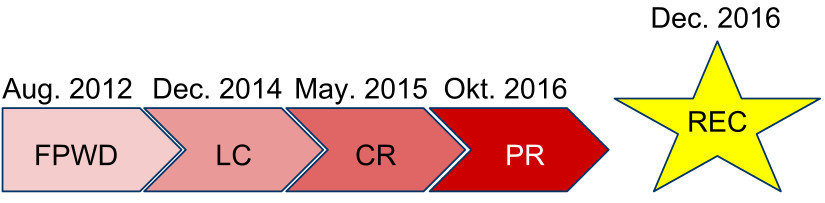
\includegraphics[width=0.95\textwidth]{pictures/roadmap.jpg}
  \caption{Roadmap zur Recommendation SVG 2.0. FPWD : First Public Working Draft,
    LC : List of Candidates,
    CR: Candidatest Recommendation,
  PR: Proposed Recommendation}
  \label{roadmap}
\end{figure}
Eine Neuerung wird sein, dass mehr CSS3 und CSS4 Befehle direkt als Attribute eingebunden werden können. Diese Attribute konnten bislang, wie bei HTML Tags üblich, auch schon über das "style"-Attribut benutzt werden. Um eine bessere Übersicht über die Möglichkeiten innerhalb eines Standards zu ermöglichen, wurde sich entschieden, die Attribute zu erweitern.\\
Zum Beispiel wird das "textoverflow" Attribut integriert. Hierbei kann der Programmierer selbst bestimmen, was mit Textbausteinen passiert, die voluminöser sind, als das vorgegebene Element. Dabei kann entschieden werden, ob diese einfach unberührt ausgeschrieben oder abgekürzt werden oder im Baustein verschwinden. \todo{Quelle}\\
Ein weiteres Beispiel ist das Farbkonzept, dass manigfaltiger im neuen Standard integriert wird. Darunter fällt nicht nur, dass mehr Farbbezeichnungen benutzt werden können, sondern auch dass der Programmierer bestimmen kann, in welchem Farbraum die Farbe kodiert und eingegeben wird.\\

Eine weitere Neuerung wird vermutlich die Integration von medialen Inhalten sein, wie Bilder, Audios, Videos, iFrames oder Canvas. Wie weiter oben erwähnt kann unter bestimmten Umständen das Canvas performanter werden. Die ganzen Elemente werden unter dem Begriff Embedded Content zusammengefasst.\\
\todo{mehr Ausblick möglich, nur bin ich schon über das Limit drüber}

\newpage


\appendix

\section{Beispiele}

\begin{figure}[h!]\centering
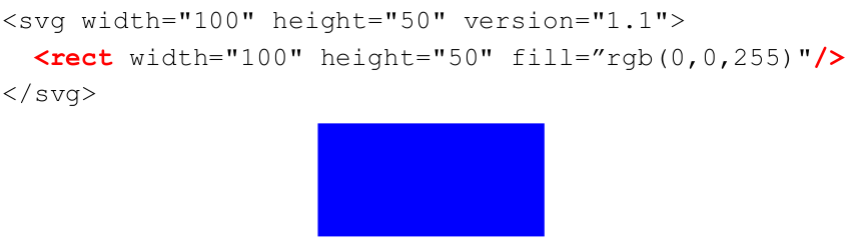
\includegraphics[width=0.6\textwidth]{pictures/rect.png}
\caption{Ein Viereck blau ausgefüllt.}
\label{fig:rect}\end{figure}
\begin{figure}[h!]\centering
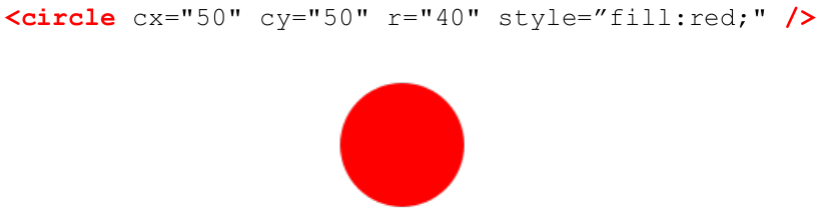
\includegraphics[width=0.6\textwidth]{pictures/circle.png}
\caption{Ein Kreis rot ausgefüllt.}
\label{fig:circle}\end{figure}
\begin{figure}[h!]\centering
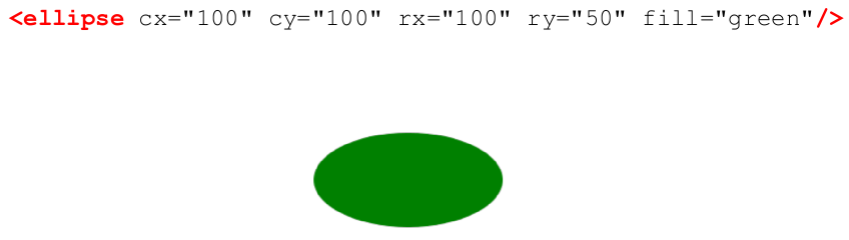
\includegraphics[width=0.6\textwidth]{pictures/ellipse.png}
\caption{Eine Ellipse grün ausgefüllt.}
\label{fig:ellipse}\end{figure}
\begin{figure}[h!]\centering
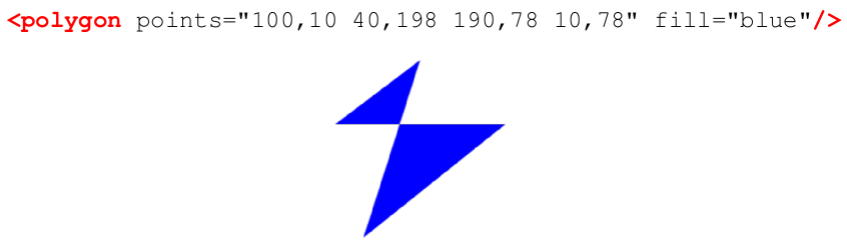
\includegraphics[width=0.6\textwidth]{pictures/polygon.png}
\caption{Beispielhaftes Polygon mit vier Punkten.}
\label{fig:poly}\end{figure}
\begin{figure}[h!]\centering
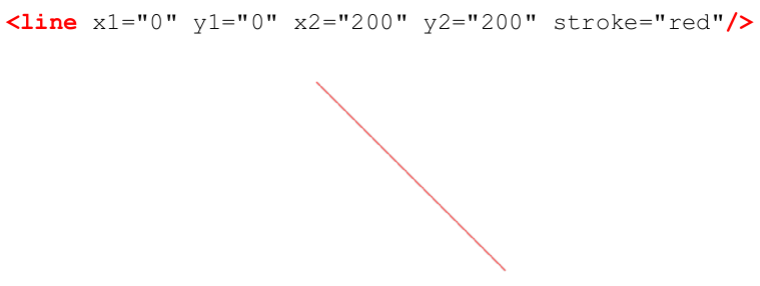
\includegraphics[width=0.6\textwidth]{pictures/line.png}
\caption{Eine einfache Linie.}
\label{fig:line}\end{figure}
\begin{figure}[h!]\centering
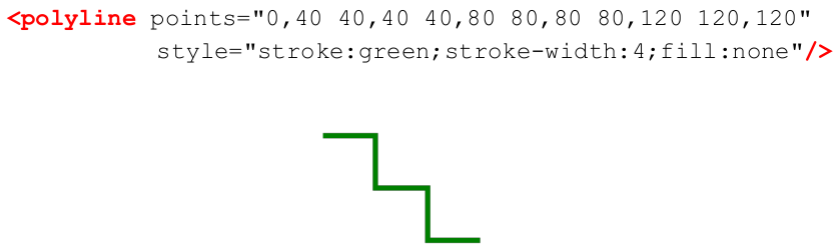
\includegraphics[width=0.6\textwidth]{pictures/polyline.png}
\caption{Einfache Polyline mit sechs Punkten.}
\label{fig:polyl}\end{figure}
\begin{figure}[h!]\centering
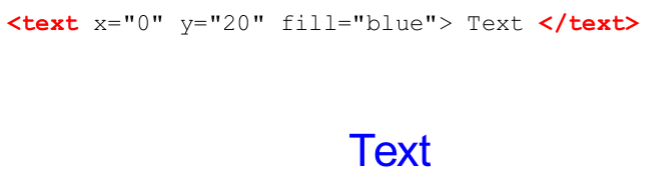
\includegraphics[width=0.6\textwidth]{pictures/text.png}
\caption{Ein einfacher Text in SVG.}
\label{fig:text}\end{figure}
\begin{figure}[h!]\centering
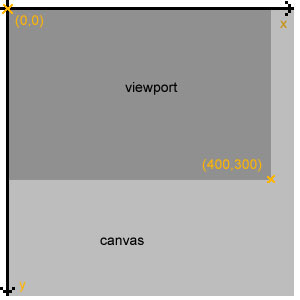
\includegraphics[width=0.3\textwidth]{pictures/koordinatensystem.jpg}
\caption{Koordinatensystem mit Canvas und Viewport.}
\label{fig:koor}\end{figure}
\begin{figure}[h!]\centering
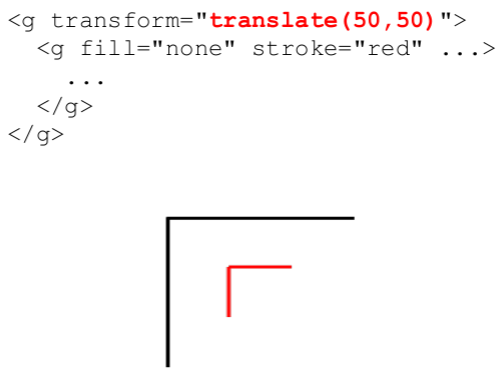
\includegraphics[width=0.6\textwidth]{pictures/transla.png}
\caption{Translation des ursprünglichen Koordinatensystems (schwarz) um jeweils 50 in x- und y-Richtung.}
\label{fig:trans}\end{figure}
\begin{figure}[h!]\centering
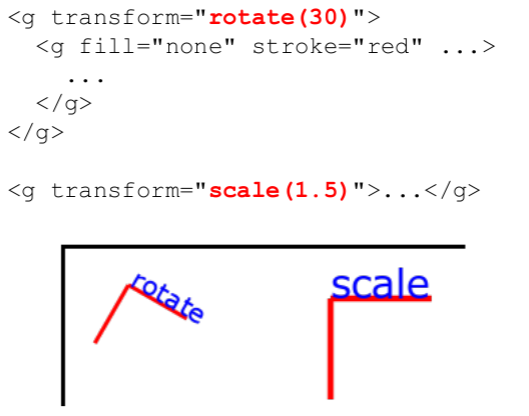
\includegraphics[width=0.6\textwidth]{pictures/rot_scal.png}
\caption{Links eine Rotation um 30. Rechts eine Vergrößerung um 1.5.}
\label{fig:rot}\end{figure}
\begin{figure}[h!]\centering
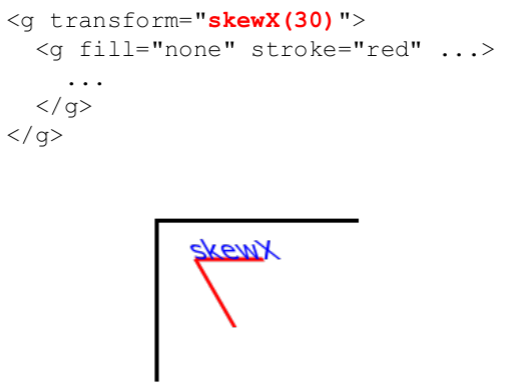
\includegraphics[width=0.6\textwidth]{pictures/skew.png}
\caption{Verzerrung um 30.}
\label{fig:skew}\end{figure}
\begin{figure}[h!]\centering
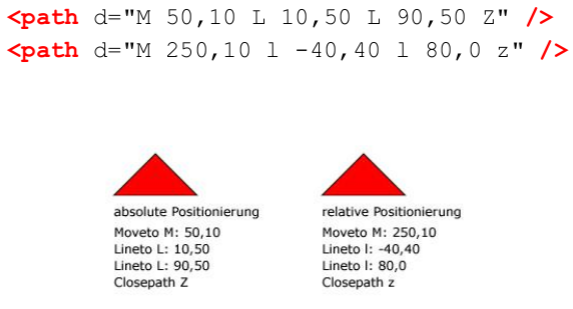
\includegraphics[width=0.6\textwidth]{pictures/path.png}
\caption{Links Pfad mit absoluter Positionierung. Rechts das gleiche Objekt mit relativer Positionierung.}
\label{fig:path}\end{figure}
\begin{figure}[h!]\centering
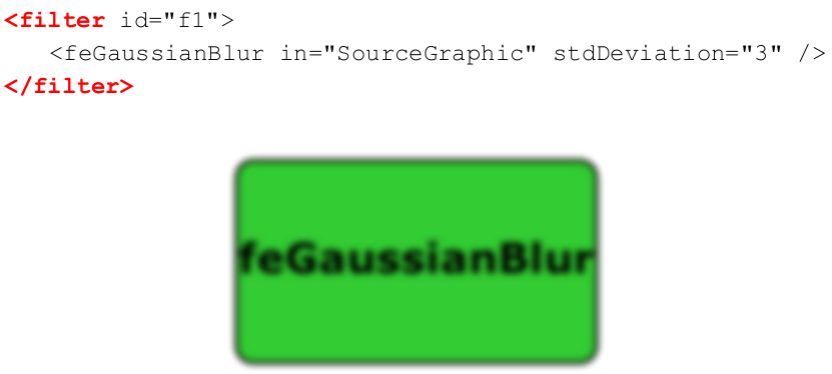
\includegraphics[width=0.6\textwidth]{pictures/filter.png}
\caption{Beispielhafter gaußscher Filter.}
\label{fig:filter}\end{figure}
\begin{figure}[h!]\centering
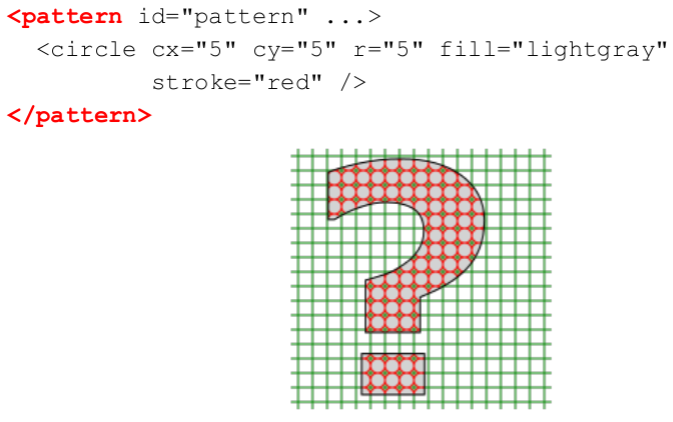
\includegraphics[width=0.6\textwidth]{pictures/pattern.png}
\caption{Das Fragezeichen wurde mit selbst definiertem Muster ausgefüllt.}
\label{fig:pattern}\end{figure}
\begin{figure}[h!]\centering
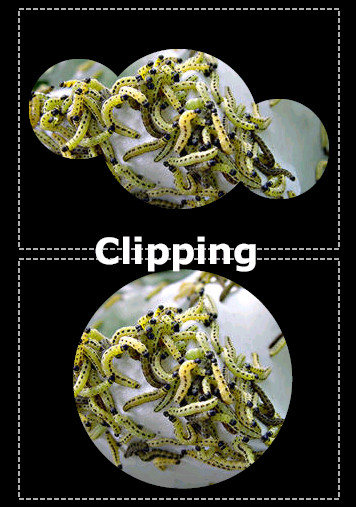
\includegraphics[width=0.3\textwidth]{pictures/kap14_1.jpg}
\caption{Beispielhaftes Clipping eines Bildes.}
\label{fig:clip}\end{figure}

\newpage

\newpage

\bibliography{sources.bib}{}
\bibliographystyle{styles/abbrvdin}

\end{document}

